\documentclass[conference]{IEEEtran}
\IEEEoverridecommandlockouts
% The preceding line is only needed to identify funding in the first footnote. If that is unneeded, please comment it out.
\usepackage{cite}
\usepackage{amsmath,amssymb,amsfonts}
\usepackage{algorithmic}
\usepackage{graphicx}
\usepackage{textcomp}
\usepackage{xcolor}
\usepackage{makecell}
\def\BibTeX{{\rm B\kern-.05em{\sc i\kern-.025em b}\kern-.08em
    T\kern-.1667em\lower.7ex\hbox{E}\kern-.125emX}}
\begin{document}

\title{Motion-Adaptive Internal Force Allocation for Dual-Arm Cooperative Manipulation // Or // Task-on-Demand Grasp Force Optimization for Dual-Arm Object Transport\\

}

\author{\IEEEauthorblockN{1\textsuperscript{st} Luca Morello}
\IEEEauthorblockA{\textit{dept. name of organization (of Aff.)} \\
\textit{name of organization (of Aff.)}\\
City, Country \\
email address or ORCID}
\and
\IEEEauthorblockN{2\textsuperscript{nd} Given Name Surname}
\IEEEauthorblockA{\textit{dept. name of organization (of Aff.)} \\
\textit{name of organization (of Aff.)}\\
City, Country \\
email address or ORCID}
\and
\IEEEauthorblockN{3\textsuperscript{rd} Given Name Surname}
\IEEEauthorblockA{\textit{dept. name of organization (of Aff.)} \\
\textit{name of organization (of Aff.)}\\
City, Country \\
email address or ORCID}
}

\maketitle

\begin{abstract}
\begin{itemize}
    \item Cooperative dual-arm transport needs enough squeeze force to prevent slip, but constant or over-conservative squeeze force wastes actuation effort and risks damaging fragile objects.
    \item We decompose the 12D dual-arm contact wrench into internal (squeeze) and external (task) components via a nullspace projection of the grasp matrix.
    \item We formulate a real-time 2-variable QP that allocates per-arm normal forces, minimizing squeeze effort and balancing the load between arms subject to friction-derived bounds.
    \item We couple the minimal grasp-force bound to the \textbf{motion state} of the manipulation task ("task-on-demand"), so the safety margin grows only while the object is in transit and relaxes at rest.
    \item We extend the same QP, at no extra decision-variable cost, with a joint-torque-aware penalty that biases squeeze-force allocation toward the arm with more actuation margin.
    \item We report internal force tracking error, friction-margin utilization, and squeeze effort with vs. without the motion-adaptive term, and with vs. without the joint-torque-aware penalty.
\end{itemize}
\end{abstract}

\begin{IEEEkeywords}
ToDo \cite{uchiyama1988symmetric}
\end{IEEEkeywords}

\section{Introduction}

\subsection{Motivation}
    \begin{itemize}
        \item Dual-arm cooperative transport needs sufficient normal (squeeze) force to prevent slip under load/inertial disturbance.
        \item Excess squeeze force is wasted actuation effort and risks damaging or destabilizing fragile/compliant objects.
        \item Human grip-force control scales with load/motion state rather than staying constant [Westling \& Johansson 1984]:  (grip force / load force coupling with friction-dependent safety margin).
    \end{itemize}

\subsection*{Positioning}
\begin{itemize}
    \item Cooperative-manipulation force-distribution literature optimizes internal force statically or per-instant, without a motion-state-dependent target.
    \item Motion/slip-adaptive grip-force literature is mostly single-gripper and slip-reactive (triggered after slip is detected/predicted), not posed as a dual-arm allocation problem.
    \item Force-distribution literature rarely couples the allocation decision back to each arm's actuation margin (joint torque headroom); it is typically treated at the end-effector/wrench level only.
\end{itemize}

\subsection*{Gap}
\begin{itemize}
    \item No existing framework couples: (a) nullspace-based internal/external wrench decomposition, (b) real-time QP allocation of squeeze force between two arms, and (c) a motion-derived force demand that is proactive (scheduled/estimated from the task's motion state) rather than reactive (slip-triggered).
    \item Joint-space actuation capacity (torque headroom, proximity to singularity/thermal limits) is not typically fed back into a real-time end-effector-level force allocator, despite the wrench-to-torque map being affine and cheap to exploit.
\end{itemize}

\subsection{What to prove}
\begin{itemize}
    \item goal of this paper is: adaptively allocating dual-arm squeeze (normal) forces based on the object’s motion can significantly improve efficiency and safety compared to a fixed safety margin.
    \item prove that coupling the minimal grasp force to the motion state (a “task-on-demand” safety margin) will reduce wasted actuation effort (and thus energy/power) without compromising slip stability.
    \item demonstrate that biasing the force allocation toward the arm with more joint torque capacity further improves overall performance
    \item \textbf{Motion-adaptive grip force reduces effort}
    \begin{itemize}
        \item  We hypothesize that tying the minimum grasp force to object velocity (instead of a constant margin) will *lower the average commanded squeeze force* and the total actuator work
        \item directly inspired by human grip behavior
        \item Likewise, adaptive grasp designs can hold objects securely with much lower forces By analogy, our motion-driven scheme should yield noticeably lower total squeeze force (hence lower power draw) than a constant-margin controller, especially when the object is at rest. 
    \end{itemize}
    \item \textbf{Slip safety is maintained when needed}
        \begin{itemize}
            \item Even though we reduce unnecessary force at rest, we expect the *dynamic slip margin* to remain safe during motion
        \end{itemize}

    \item \textbf{Balanced load and torque awareness}
        \begin{itemize}
            \item Our QP also enforces balanced force distribution (penalizing one arm doing all the work) and can include a joint-torque cost.
            \item We hypothesize that adding the torque-aware quadratic terms will shift squeeze effort onto the arm with more actuation headroom.
            This should *increase each arm’s torque margin* (distance to its limits) relative to a force-unaware allocation.
        \end{itemize}
\end{itemize}

\subsection{Contributions}
\begin{itemize}
    \item a two-variable QP can allocate normal forces to both arms in real time while enforcing friction and actuation bounds
    \item making the safety floor velocity-dependent (task-on-demand) measurably reduces overall effort
    \item adding a small torque-penalty reshapes the force split to protect the arm with tighter joint capacity
    \item We will contrast each element against simpler baselines (e.g. fixed safety margin, no torque cost) and show the improvements in clear metrics.  
\end{itemize}


\section{Related Work}

\subsection{Internal/external force decomposition and QP-based load distribution}
\begin{itemize}
    \item Classical hybrid two-arm coordination and internal/external wrench split (Uchiyama \& Dauchez).
    \item QP-based minimization of internal forces in cooperating manipulators (Nahon \& Angeles, 1992).
    \item NLP/QP force-distribution schemes with normal-force constraints (Kwon \& Lee; Kazerooni).
    \item Recent result: non squeezing internal load distributions from a generalized inverse of the grasp matrix are \textbf{not unique}
    \item Admittance/QP dual-arm cobot frameworks regulating internal vs. external effort for safe bimanual interaction (BAZAR-style hierarchical QP).
\end{itemize}

\subsection{Friction-cone-constrained grasp/contact force optimization}
\begin{itemize}
    \item Canonical exact formulation: friction-cone feasibility as positive-definiteness / SDP (Buss, Hashimoto \& Moore, 1996).
    \item Polyhedral/linear approximations of the friction cone for LP/QP tractability (Kerr \& Roth; Cheng \& Orin).
\end{itemize}

\subsection{Motion and slip-adaptive grip force control}
\begin{itemize}
    \item Biological grounding: grip force/load force coordination and friction-dependent safety margin (Westling \& Johansson, 1984).
    \item Trajectory modulation as an alternative (not just complement) to grip-force modulation for slip prevention (Nature Machine Intelligence, 2025)  \\ \textbf{contrast}: this paper treats grip force as the adaptive variable and trajectory as given, the inverse framing.
    \item Human hand-acceleration modulation alongside grip-force modulation for slip prevention (2024 study) \\  \textbf{motivates} a velocity/acceleration-estimated demand term.
    \item Reactive slip control via internal-force optimization for multifingered hands, arguing uniform force increases perturb object pose vs. allocation-aware optimization (Théo Ayral)
\end{itemize}



\section{System Overview}
\subsection{Platform and FSM}
\begin{itemize}
    \item Dual xArm7 setup in mc\_rtc.
    \item FSM: Idle → Independent (reach) → Collaborative { Build-Grasp → Trajectory → Cooperative Motion }.
    \item One system-diagram figure.
\end{itemize}

\subsection{Problem Statement}
\begin{itemize}
    \item At every control cycle, find the per-arm normal (squeeze) forces
    \begin{align}
                \mathbf{x} = \begin{bmatrix}
            F_{n,L} \\
            F_{n,R}
        \end{bmatrix}
    \end{align}

    that:
    \begin{itemize}
        \item track a desired internal grasp force level,
        \item respect friction-derived and actuation bounds,
        \item remain balanced between the two arms,
    \end{itemize}
\end{itemize}

\section{Internal Wrench Decomposition and Squeeze Isolation}

\subsection*{System Wrench and Grasp Matrix}
\begin{itemize}
    \item dual-arm wrench $w\in \mathbb{R}^{1\times12}$:
    \begin{align}
        w &=
        \begin{bmatrix}
            w_L \\
            w_R
        \end{bmatrix}
        \in \mathbb{R}^{12},
    \end{align}
    where \(w_L = [\tau_L; f_L]\) and \(w_R = [\tau_R; f_R]\).

    \item Grasp matrix \(G \in \mathbb{R}^{6 \times 12}\) and internal-wrench nullspace projector:
    \begin{align}
        P_{\mathrm{int}} = I_{12} - G^\dagger G.
    \end{align}

    \item Internal wrench:
    \begin{align}
        w_{\mathrm{int}} = P_{\mathrm{int}}\, w.
    \end{align}
\end{itemize}

\subsection{Squeeze Subspace Isolation}

\begin{itemize}
    \item defined the squeeze direction $n_s$ 

    \item Let \(N\) denote the orthonormal nullspace basis of \(G\), obtained via singular value decomposition (SVD).

    \item Normalized, kinematically valid squeeze direction:
    \begin{align}
        n_{\mathrm{squeeze}}
        =
        \frac{N N^{T} n_s}
        {\left\lVert N N^{T} n_s \right\rVert}.
    \end{align}
\end{itemize}

\subsection{Scalar Grasp Force}
\begin{itemize}
    \item The grasp-force scalar is given by
    \begin{align}
        \lambda_{\mathrm{grasp}}
        &= n_{\mathrm{squeeze}}^{T} w_{\mathrm{int}} \\
        &= n_{\mathrm{squeeze}}^{T} P_{\mathrm{int}}\, w.
    \end{align}

    \item Since \(n_{\mathrm{squeeze}} \in \mathcal{N}(G)\), it follows that
    \(P_{\mathrm{int}} n_{\mathrm{squeeze}} = n_{\mathrm{squeeze}}\). Moreover,
    \(P_{\mathrm{int}}\) is an orthogonal projector and is therefore symmetric,
    i.e., \(P_{\mathrm{int}}^{T} = P_{\mathrm{int}}\). Hence,
    \begin{align}
        \lambda_{\mathrm{grasp}}
        &= n_{\mathrm{squeeze}}^{T} P_{\mathrm{int}}\, w \\
        &= \left(P_{\mathrm{int}} n_{\mathrm{squeeze}}\right)^{T} w \\
        &= n_{\mathrm{squeeze}}^{T} w.
    \end{align}

    \item This identity shows that only the component of \(w\) lying in the
    internal-wrench subspace contributes to \(\lambda_{\mathrm{grasp}}\); any
    object-motion wrench is orthogonal to \(n_{\mathrm{squeeze}}\).
\end{itemize}

\subsection{Decomposing $w$ into Fixed and Optimized Parts}
\begin{itemize}
    \item The total contact wrench is decomposed as
    \begin{align}
        w = w_{\mathrm{fixed}} + S_n x,
    \end{align}
    where \(w_{\mathrm{fixed}}\) contains the measured contact moments and
    tangential forces (which are not optimized), and
    \(S_n \in \mathbb{R}^{12 \times 2}\) maps the decision variables to the
    world-frame normal-force wrench components through the unit contact normals
    \(\hat{u}_L\) and \(\hat{u}_R\).

    \item Substituting the above decomposition into
    \(\lambda_{\mathrm{grasp}} = n_{\mathrm{squeeze}}^{T} w\) yields the affine
    grasp-force model:
    \begin{align}
        \lambda_{\mathrm{grasp}}(x)
        &= c^{T} x + \lambda_{0},
    \end{align}
    where
    \begin{align}
        c^{T} &= n_{\mathrm{squeeze}}^{T} S_n, \\
        \lambda_{0} &= n_{\mathrm{squeeze}}^{T} w_{\mathrm{fixed}}.
    \end{align}

    \item The coefficients \(c_L\) and \(c_R\) quantify the contribution of a
    unit normal force applied by the left and right manipulators,
    respectively, to the internal squeeze force. The offset
    \(\lambda_{0}\) represents the squeeze already generated by the fixed
    contact moments and tangential force components.
\end{itemize}


\section{Motion-Adaptive Force Demand}

\subsection{Motivation}

\begin{itemize}
    \item The constant safety-margin approach provides a simple baseline but ignores the dynamic state of the manipulation task. Consequently, the same minimum grasp force is maintained regardless of whether the object is stationary or undergoing rapid motion.

    \item During transport, inertial effects, transient disturbances, and tracking errors increase the likelihood of relative motion between the object and the grippers. Conversely, when the object is at rest, maintaining the same force is unnecessarily conservative and may increase energy consumption and contact pressure.

    \item The objective is therefore to design a motion-adaptive force demand that automatically increases the minimum allowable grasp force during object motion while relaxing it as the object approaches rest.

    \item The resulting formulation should satisfy the following design requirements:
    \begin{itemize}
        \item Zero force demand at rest.
        \item Smooth and continuous evolution during motion.
        \item Bounded output with a configurable maximum force.
        \item Independence from a particular trajectory generator.
    \end{itemize}
\end{itemize}


\subsection{Velocity-Based Motion Index}

\begin{itemize}

    \item Several motion indicators were considered for adapting the grasp-force demand.

    \item Acceleration was initially investigated since inertial loading is directly related to acceleration. However, the acceleration profile of common point-to-point trajectories exhibits a characteristic double-lobe shape, becoming zero at the midpoint where the object reaches its maximum velocity. This behavior undesirably reduces the predicted force demand exactly when the object is still undergoing significant dynamic motion.

    \item Instead, the object translational velocity is adopted as the scheduling variable. Velocity evolves smoothly throughout the transport phase, reaches a single maximum during the trajectory, and naturally returns to zero only at the beginning and end of the motion.

    \item Furthermore, the velocity signal can be obtained directly from robot measurements, making the formulation independent of any specific trajectory parameterization or planner timing law.
    \item The proposed scheduler is purely measurement-driven and therefore does not require access to trajectory timing variables or planner-specific information.
\end{itemize}

The estimated object translational velocity is computed as the average of the measured end-effector linear velocities

\begin{align}
v_{\mathrm{obj}}
=
\frac{1}{2}
\left(
\dot{x}_L+\dot{x}_R
\right),
\end{align}

whose magnitude is

\begin{align}
v
=
\left\|
v_{\mathrm{obj}}
\right\|.
\end{align}

To prevent sensor noise and low-amplitude oscillations from activating the adaptive force, a deadband is introduced,

\begin{align}
v_{\mathrm{eff}}
=
\max\left(0,\,
v-v_{\mathrm{db}}
\right),
\end{align}

where $v_{\mathrm{db}}$ denotes the velocity threshold below which the object is considered stationary.


\subsection{Raised-Cosine Force Scheduling}

\begin{itemize}

    \item Rather than scaling the demanded force linearly with velocity, a nonlinear activation function is employed.

    \item The chosen function is a raised cosine, which provides a smooth transition from zero to one while remaining continuously differentiable over its entire domain.

    \item The function naturally saturates at unity, allowing the maximum demanded force to be specified explicitly without requiring additional saturation operators.

    \item A shape parameter allows the designer to tune how aggressively the force increases with motion. Smaller values produce a faster initial rise, whereas larger values delay the increase until higher object velocities are reached.

    \item Since the activation depends solely on measured velocity, the formulation remains independent of trajectory generators and can be applied to arbitrary motion planners.
\end{itemize}

The normalized velocity is first computed as

\begin{align}
z
=
\mathrm{clip}
\left(
\frac{v_{\mathrm{eff}}}{\delta},
0,
1
\right),
\end{align}

where $\delta$ defines the Activation Threshold velocity at which the adaptive force reaches its maximum.

The motion activation coefficient is then defined by the raised-cosine function

\begin{align}
\alpha(v)
=
\frac{1}{2}
\left(
1-
\cos
\left(
\pi z^k
\right)
\right),
\end{align}

where $k>0$ controls the curvature of the transition.

Finally, the motion-adaptive force demand is computed as

\begin{align}
F_{\mathrm{demand}}
=
F_{\max}\,
\alpha(v),
\end{align}

where $F_{\max}$ represents the maximum additional force contribution permitted by the scheduler.


\begin{figure}[htbp]
\centerline{
\includegraphics[width=0.85\columnwidth]{imgs/Activation.png}}
\caption{illustrates the evolution of the activation function for different values of the shape parameter $k$. As the object begins moving, the demanded force increases smoothly from zero, gradually approaching $F_{\max}$ as the velocity reaches the characteristic value $L$. This smooth scheduling avoids discontinuities while providing greater grasp stability during dynamic manipulation than a constant safety-margin strategy.}
\label{cosine}
\end{figure}

\begin{itemize}


    \item The deadband prevents small velocity fluctuations caused by sensing noise or controller regulation from unnecessarily increasing the grasp force.

    \item The characteristic velocity $L$ determines the operating range of the scheduler, while the exponent $k$ controls the sensitivity of the transition, allowing straightforward tuning for different manipulation tasks.

\end{itemize}


\section{QP Formulation for Squeeze Force Optimization}

\subsection{Cost Function}
\begin{equation}
\begin{aligned}
J(x)
=\;
&\alpha\big(\lambda_{\mathrm{grasp}}(x)-\lambda_{\mathrm{reference}}(t)\big)^2
+\beta\,(F_{n,L}-F_{n,R})^2 \\
&+\gamma_L\lVert\tau_{c,L}(x)\rVert^2
+\gamma_R\lVert\tau_{c,R}(x)\rVert^2,
\qquad \alpha,\beta,\gamma_L,\gamma_R>0.
\end{aligned}
\label{eq:cost_full}
\end{equation}

\begin{equation}
\lambda_{\mathrm{reference}}(t) = \lambda_{\mathrm{base}} + F_{\mathrm{demand}}\big(v(t)\big),
\label{eq:lambda_ref}
\end{equation}

where $\lambda_{\mathrm{base}}$ is a constant, configurable baseline squeeze level and $F_{\mathrm{demand}}(v)$ is the motion-adaptive term of Section~\ref{sec:motion_demand}. This choice is not cosmetic: the per-arm lower bounds derived in Section~\ref{sec:constraints} already enforce the minimum compression required for non-slip, so if the cost simply minimized $\lambda_{\mathrm{grasp}}$ the optimum would always sit on that bound regardless of $\gamma_L,\gamma_R$, leaving the torque-aware terms with no effect on the solution. Tracking a reference above the bound gives the optimizer slack to trade squeeze force against joint-torque effort while still meeting the motion-dependent force demand.

The remaining terms are as before: the balance term $\beta(F_{n,L}-F_{n,R})^2$ discourages one arm from carrying a disproportionate share of the grasp load, and the torque terms $\gamma_L\lVert\tau_{c,L}(x)\rVert^2$, $\gamma_R\lVert\tau_{c,R}(x)\rVert^2$ penalize the joint torques required to realize the commanded contact wrenches, biasing the allocation toward the arm with more actuation headroom when $\gamma_L\neq\gamma_R$.

The objective function is designed to achieve three complementary goals: regulating the desired internal grasp force, promoting balanced load sharing between the manipulators, and reducing the joint-space effort required to realize the resulting contact-force distribution. 
The first term penalizes the deviation between the internal grasp force, $\eta_{\mathrm{grasp}}(x)$, computed from the contact-force decomposition, and its desired reference value, $\eta_{\mathrm{reference}}$. 
The second term minimizes the difference between the normal contact forces at the left and right contacts, encouraging a balanced distribution of the grasp load and preventing one manipulator from carrying a disproportionate share of the required squeezing force.
Although the optimization is formulated in terms of end-effector contact wrenches, the resulting joint torques depend on the robot configuration. The final two terms therefore introduce a quadratic penalty on the commanded joint torques of the left and right manipulators. The commanded joint torques are obtained from the end-effector wrenches through

\begin{align}
\tau = J^{T}w,
\end{align}
where $J$ denotes the manipulator Jacobian and $w$ is the commanded end-effector wrench. Since $w$ is an affine function of the optimization variable $x$, the joint torques are likewise affine in $x$, allowing the torque regularization to be incorporated directly into the quadratic objective without introducing additional decision variables or modifying the structure of the optimization problem.

The weighting coefficients $\alpha$, $\beta$, $\gamma_L$, and $\gamma_R$ determine the relative importance of the three objectives. Specifically, $\alpha$ regulates the trade-off between achieving the desired internal grasp force and limiting the overall squeeze effort, while $\beta$ determines the emphasis placed on balanced load sharing. The coefficients $\gamma_L$ and $\gamma_R$ govern the influence of the joint-torque regularization for the left and right manipulators, respectively. Equal values promote a symmetric distribution of joint effort, whereas asymmetric values can intentionally bias the force allocation toward the manipulator with greater available actuation capacity, for example when the opposite arm is operating closer to a singular configuration, joint torque limit, or thermal constraint.

\subsection{Per-Arm Affine Torque Map}

Because the normal force commanded at one contact produces a wrench only at that contact, the mapping $S_n$ introduced in Section~\ref{sec:decomposition} is block-diagonal,
\begin{equation}
S_n =
\begin{bmatrix}
S_{n,L} & 0 \\
0 & S_{n,R}
\end{bmatrix}
\in\mathbb{R}^{12\times2},
\qquad S_{n,L},S_{n,R}\in\mathbb{R}^{6},
\end{equation}
so that $w_L = w_{\mathrm{fixed},L} + S_{n,L}F_{n,L}$ and $w_R = w_{\mathrm{fixed},R}+S_{n,R}F_{n,R}$ depend only on their own arm's decision variable. Mapping each contact wrench to joint torques through the arm Jacobian, $\tau_{c,L}(x)=J_L^{T}w_L$ and $\tau_{c,R}(x)=J_R^{T}w_R$, gives the affine, decoupled form
\begin{align}
\tau_{c,L}(x) &= \tau_{\mathrm{fixed},L} + b_L\,F_{n,L}, &
b_L &= J_L^{T}S_{n,L}, \\
\tau_{c,R}(x) &= \tau_{\mathrm{fixed},R} + b_R\,F_{n,R}, &
b_R &= J_R^{T}S_{n,R},
\end{align}
with $\tau_{\mathrm{fixed},L}=J_L^{T}w_{\mathrm{fixed},L}$, $\tau_{\mathrm{fixed},R}=J_R^{T}w_{\mathrm{fixed},R}$. Since $\tau_{c,L}$ depends only on $F_{n,L}$ (and likewise for $R$), the torque penalty contributes only diagonal terms to the QP Hessian, as shown next.

\subsection{Standard QP Form Derivation}
\label{sec:qp_derivation}

As in Section~\ref{sec:decomposition}, the grasp force is affine in $x=[F_{n,L},F_{n,R}]^{T}$,
\begin{equation}
\lambda_{\mathrm{grasp}}(x) = c^{T}x+\lambda_0,
\qquad
c^{T}=n_{\mathrm{squeeze}}^{T}P_{\mathrm{int}}S_n,
\qquad
\lambda_0 = n_{\mathrm{squeeze}}^{T}P_{\mathrm{int}}w_{\mathrm{fixed}}.
\end{equation}

Substituting the reference of \eqref{eq:lambda_ref}, define the reference-shifted offset
\begin{equation}
\tilde\lambda_0(t) \;:=\; \lambda_0 - \lambda_{\mathrm{reference}}(t),
\end{equation}
so that the tracking error is again affine, $\lambda_{\mathrm{grasp}}(x)-\lambda_{\mathrm{reference}}(t)=c^{T}x+\tilde\lambda_0$, and

\begin{equation}
\big(\lambda_{\mathrm{grasp}}(x)-\lambda_{\mathrm{reference}}\big)^2
= x^{T}cc^{T}x + 2\tilde\lambda_0\,c^{T}x + \tilde\lambda_0^{2}.
\end{equation}

With $d=[1,-1]^{T}$, the balance term expands, as before, to $x^{T}dd^{T}x$ with no linear contribution. For the torque terms, squaring the affine maps of the previous subsection gives
\begin{align}
\lVert\tau_{c,L}(x)\rVert^2 &= \lVert\tau_{\mathrm{fixed},L}\rVert^2 + 2F_{n,L}\big(\tau_{\mathrm{fixed},L}\cdot b_L\big) + F_{n,L}^{2}\lVert b_L\rVert^2, \\
\lVert\tau_{c,R}(x)\rVert^2 &= \lVert\tau_{\mathrm{fixed},R}\rVert^2 + 2F_{n,R}\big(\tau_{\mathrm{fixed},R}\cdot b_R\big) + F_{n,R}^{2}\lVert b_R\rVert^2.
\end{align}

Collecting all quadratic and linear terms in $x$ and dropping the constants ($\tilde\lambda_0^2$, $\lVert\tau_{\mathrm{fixed},L}\rVert^2$, $\lVert\tau_{\mathrm{fixed},R}\rVert^2$), the cost matches the standard QP form
\begin{equation}
J(x) = \tfrac{1}{2}x^{T}Hx + g^{T}x,
\end{equation}
with
\begin{equation}
H = 2
\begin{bmatrix}
\alpha c_L^{2}+\beta+\gamma_L\lVert b_L\rVert^2 &
\alpha c_Lc_R-\beta \\[4pt]
\alpha c_Lc_R-\beta &
\alpha c_R^{2}+\beta+\gamma_R\lVert b_R\rVert^2
\end{bmatrix},
\label{eq:H_full}
\end{equation}
\begin{equation}
g =
2\begin{bmatrix}
\alpha\tilde\lambda_0\,c_L + \gamma_L\big(\tau_{\mathrm{fixed},L}\cdot b_L\big) \\[4pt]
\alpha\tilde\lambda_0\,c_R + \gamma_R\big(\tau_{\mathrm{fixed},R}\cdot b_R\big)
\end{bmatrix}.
\label{eq:g_full}
\end{equation}

The reference-tracking and balance terms couple $F_{n,L}$ and $F_{n,R}$ through the off-diagonal entry $\alpha c_Lc_R-\beta$, while the torque penalty enters only on the diagonal, consistent with the per-arm decoupling established above. Increasing $\gamma_L$ relative to $\gamma_R$ stiffens the left diagonal entry and its corresponding gradient term, shifting the optimal split of squeeze force toward the right arm without changing the problem's dimension or the coupling structure introduced by $\alpha$ and $\beta$.
\subsection{Constraints}
\label{sec:constraints}

The decision variables are signed contact-normal forces, with a negative value denoting compression along the inward contact normal (i.e. squeezing) and values closer to zero denoting a lighter grasp. Under this convention, \emph{more} negative means \emph{more} compressive force, so a minimum-compression requirement becomes an \emph{upper} bound on $x$, while the actuation limit becomes a \emph{lower} bound.

The upper bound is derived from the Coulomb friction limit at each contact, using the measured tangential (in-plane) force component:
\begin{equation}
x_u^L(t) = -\frac{|F_{t,L}(t)|}{\mu} - \delta,
\qquad
x_u^R(t) = -\frac{|F_{t,R}(t)|}{\mu} - \delta,
\label{eq:friction_bound}
\end{equation}
where $F_{t,L},F_{t,R}$ are the measured tangential force components at the left and right contacts, $\mu$ is the friction coefficient, and $\delta\ge0$ is a fixed safety margin. As with the earlier friction constraint, $F_{t,L}$ and $F_{t,R}$ are taken from the current sensor sample, which reflects the previously commanded contact wrench — the same deliberate one-cycle lag noted in Section~\ref{sec:decomposition}. In the present implementation $\mu$ and $\delta$ are shared between the two arms; per-arm $\mu_L,\mu_R$ is a straightforward extension.

The lower bound $x_l$ is a fixed, conservative actuation floor common to both arms (e.g. a hardware- or safety-rated force limit), independent of the sensed tangential force. The resulting box constraints are
\begin{equation}
x_l \le F_{n,L} \le x_u^L(t),
\qquad
x_l \le F_{n,R} \le x_u^R(t).
\label{eq:box_constraints}
\end{equation}

\emph{Remark.} $\lambda_{\mathrm{reference}}(t)$ in \eqref{eq:lambda_ref} and the bound \eqref{eq:friction_bound} are computed independently: the bound guarantees non-slip in the worst case, while the reference sets the desired operating point beyond it. In the current implementation $\lambda_{\mathrm{base}}$ and $F_{\mathrm{demand}}$ are tuned so that the commanded total squeeze magnitude stays comfortably above $|x_u^L(t)|+|x_u^R(t)|$ across the tested trajectories. Explicitly coupling the two — e.g. defining the reference relative to the instantaneous bound,
\begin{equation}
\lambda_{\mathrm{reference}}(t) = \big(|x_u^L(t)|+|x_u^R(t)|\big) + \mathrm{SM}_{\mathrm{target}},
\end{equation}
with $\mathrm{SM}_{\mathrm{target}}\ge0$ a configurable target safety margin beyond the friction limit — is a natural refinement left for future work, since it would make the reference itself slip-aware rather than only motion-aware.

\subsection{Final Problem}

At every control cycle the allocator solves
\begin{equation}
\min_{x}\ \tfrac{1}{2}x^{T}Hx+g^{T}x
\quad\text{s.t.}\quad
x_l \le F_{n,L} \le x_u^L(t),\;\;
x_l \le F_{n,R} \le x_u^R(t),
\end{equation}
with $H$ and $g$ given in \eqref{eq:H_full}–\eqref{eq:g_full}. The problem remains a two-variable, box-constrained QP regardless of the torque-aware extension, so the real-time solve cost is unchanged from the base allocator.







\section{Experimental Validation}



\subsection{Platform and Protocol}

\begin{itemize}
    \item Dual xArm7, \texttt{mc\_rtc}.

    \item Pick--carry--place trajectory; force-demand conditions:
    \begin{itemize}
        \item (a) constant \texttt{F\_static} baseline,
        \item (b) schedule-driven \texttt{F\_demand},
        \item (c) motion-estimated \texttt{F\_demand},
        \item (d) hybrid.
    \end{itemize}

    \item Torque-awareness conditions: with vs. without the extension, symmetric vs. asymmetric \(\gamma_L,\gamma_R\).

\end{itemize}

\subsection{Metrics}

\begin{itemize}
    \item Internal force
    \item Peak/RMS tangential force relative to the friction bound (slip-margin proxy).
    \item Total squeeze effort \(\int \lVert x\rVert\,dt\).
    \item Peak/RMS joint torque per arm, and margin-to-limit, with vs. without extension.
    \item QP solve time distribution
\end{itemize}

\subsection{Figures}

\begin{itemize}
    \item FSM / system diagram.
    \item Internal force vs. trajectory phase, with all demand conditions overlaid.
    \item Friction-margin utilization over the trajectory.
    \item Joint torque per arm, with vs. without torque-aware weighting, under an induced asymmetric-capacity scenario.
    \item Contact-loss / activation-blend before-after comparison.
    \item Solve-time histogram.
\end{itemize}

\begin{figure}[htbp]
\centerline{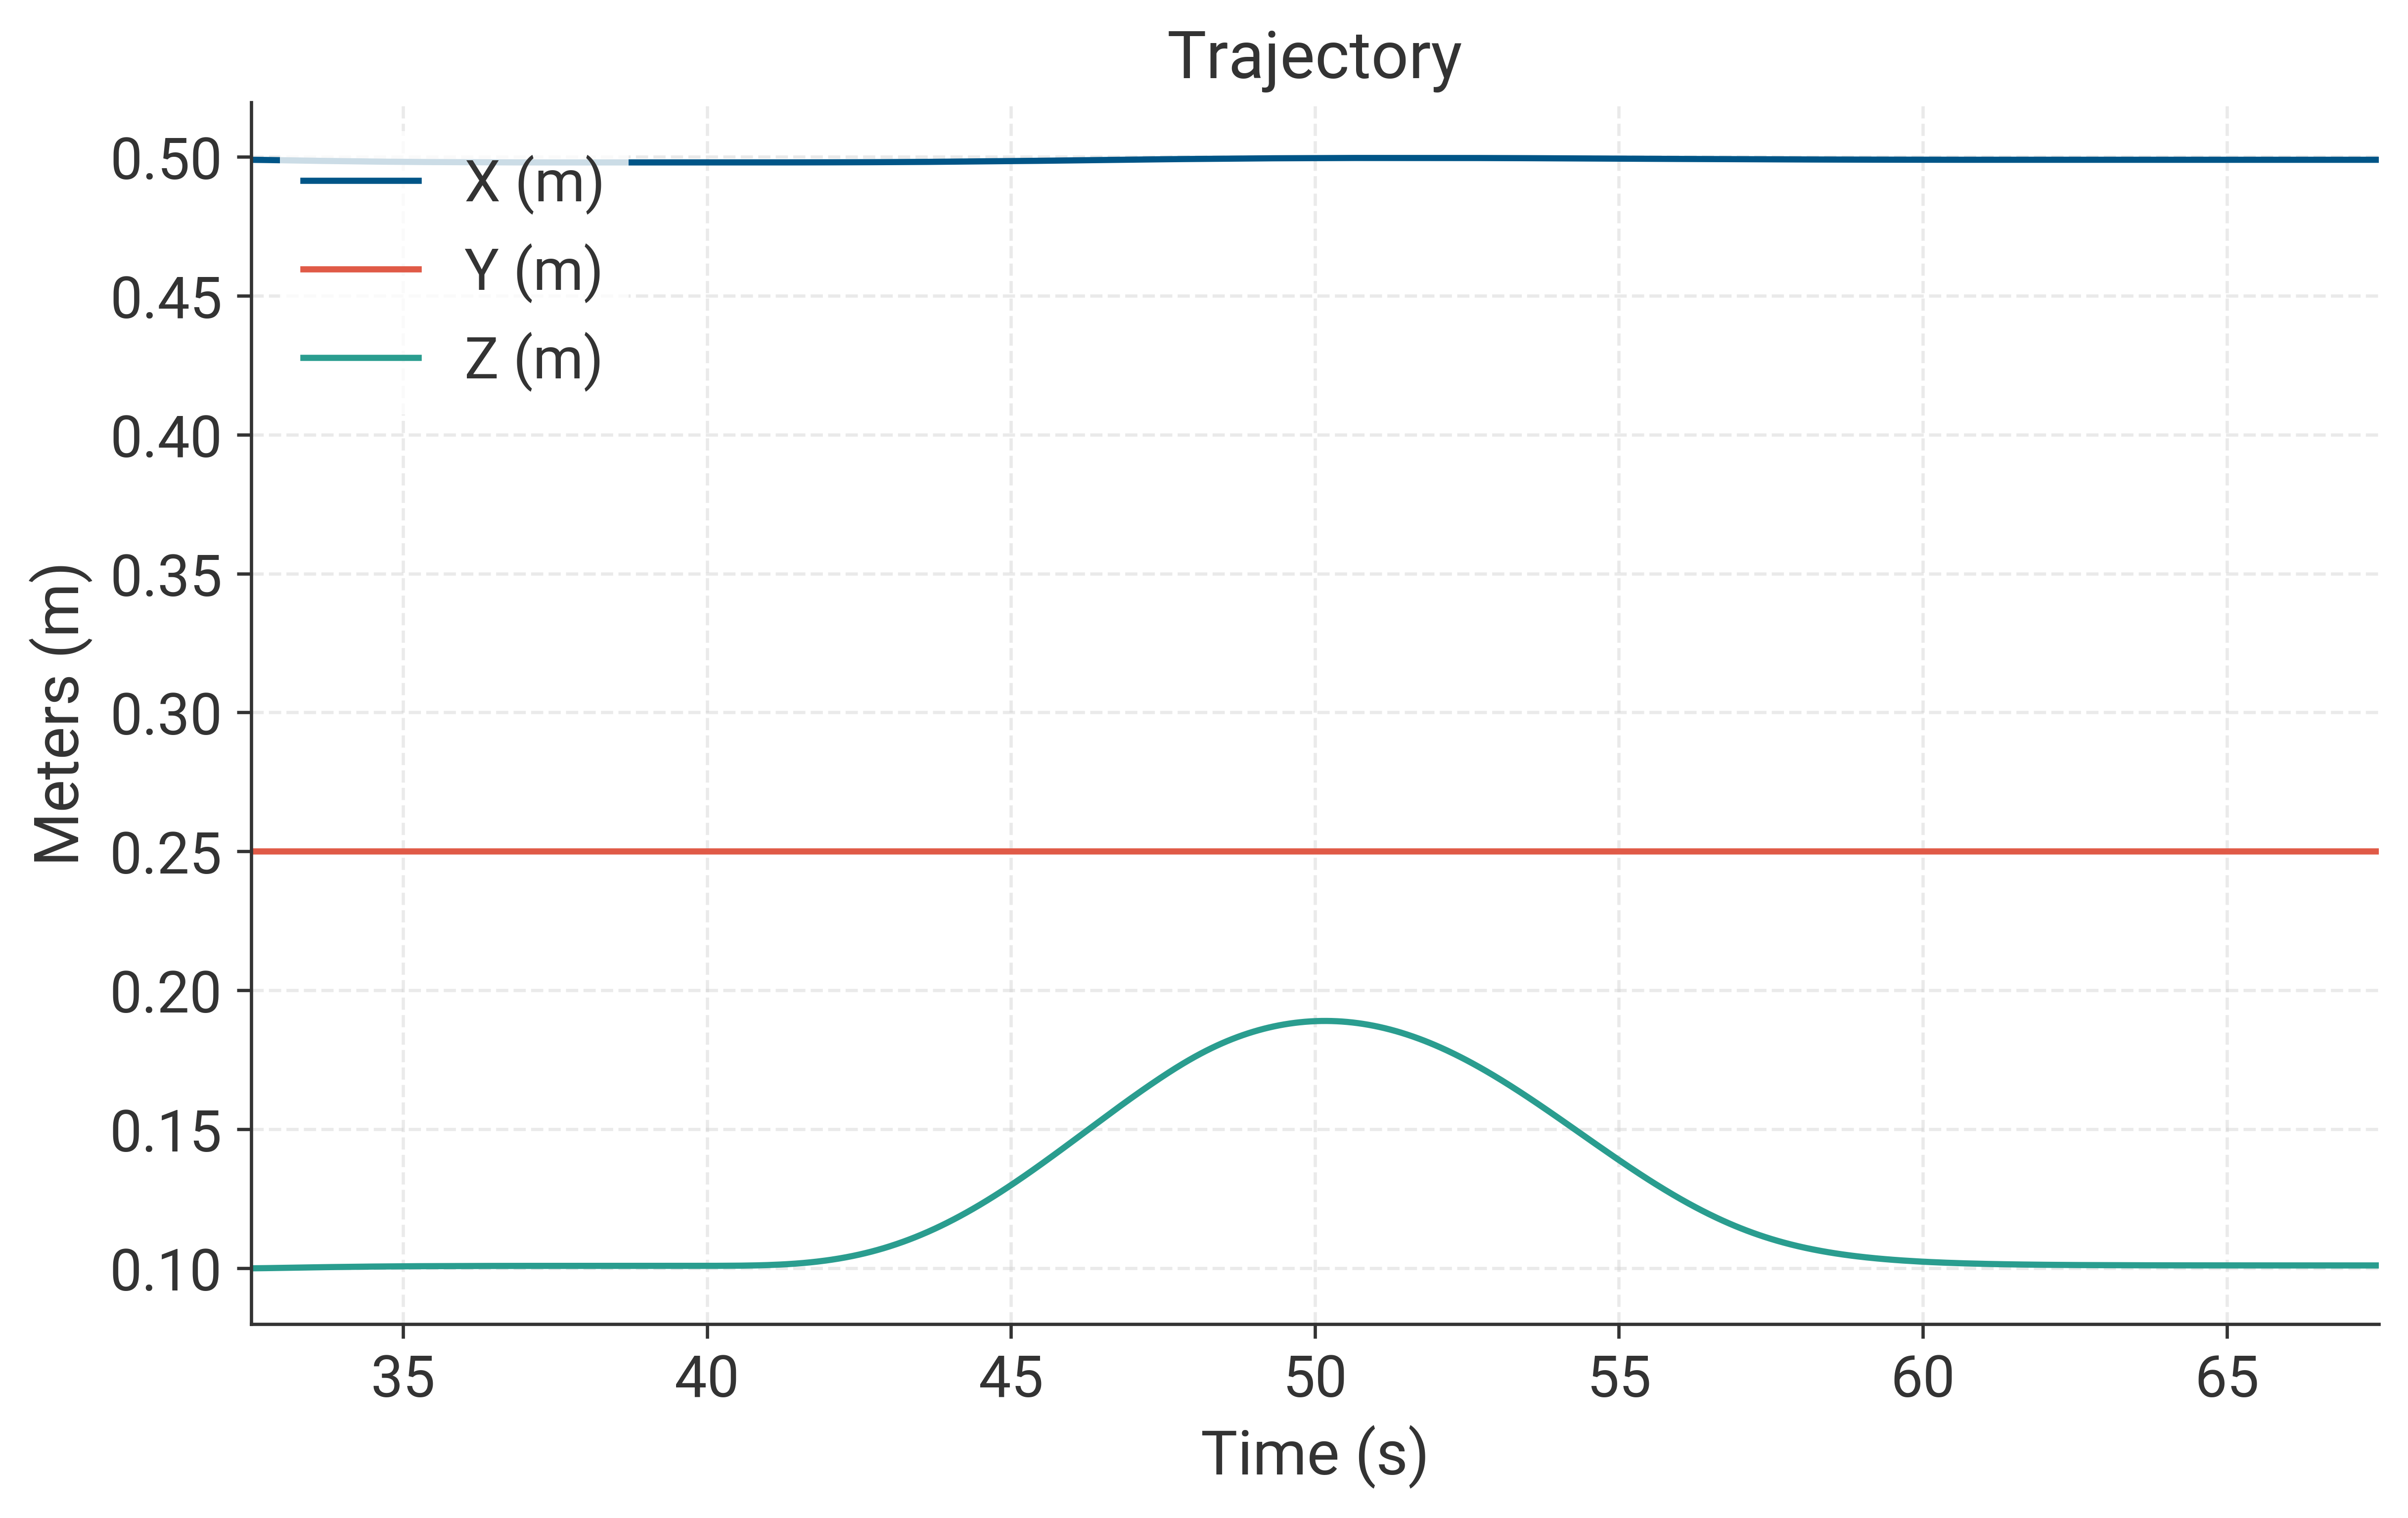
\includegraphics[width=0.85\columnwidth]{imgs/ObjectTrajecory.png}}
\caption{Kinematic results for the object. (a) Trajectory of the object, (b) velocity profile, and (c) acceleration profile during the motion.}
\label{ObjectTrajecory}
\end{figure}

\begin{figure}[htbp]
\centerline{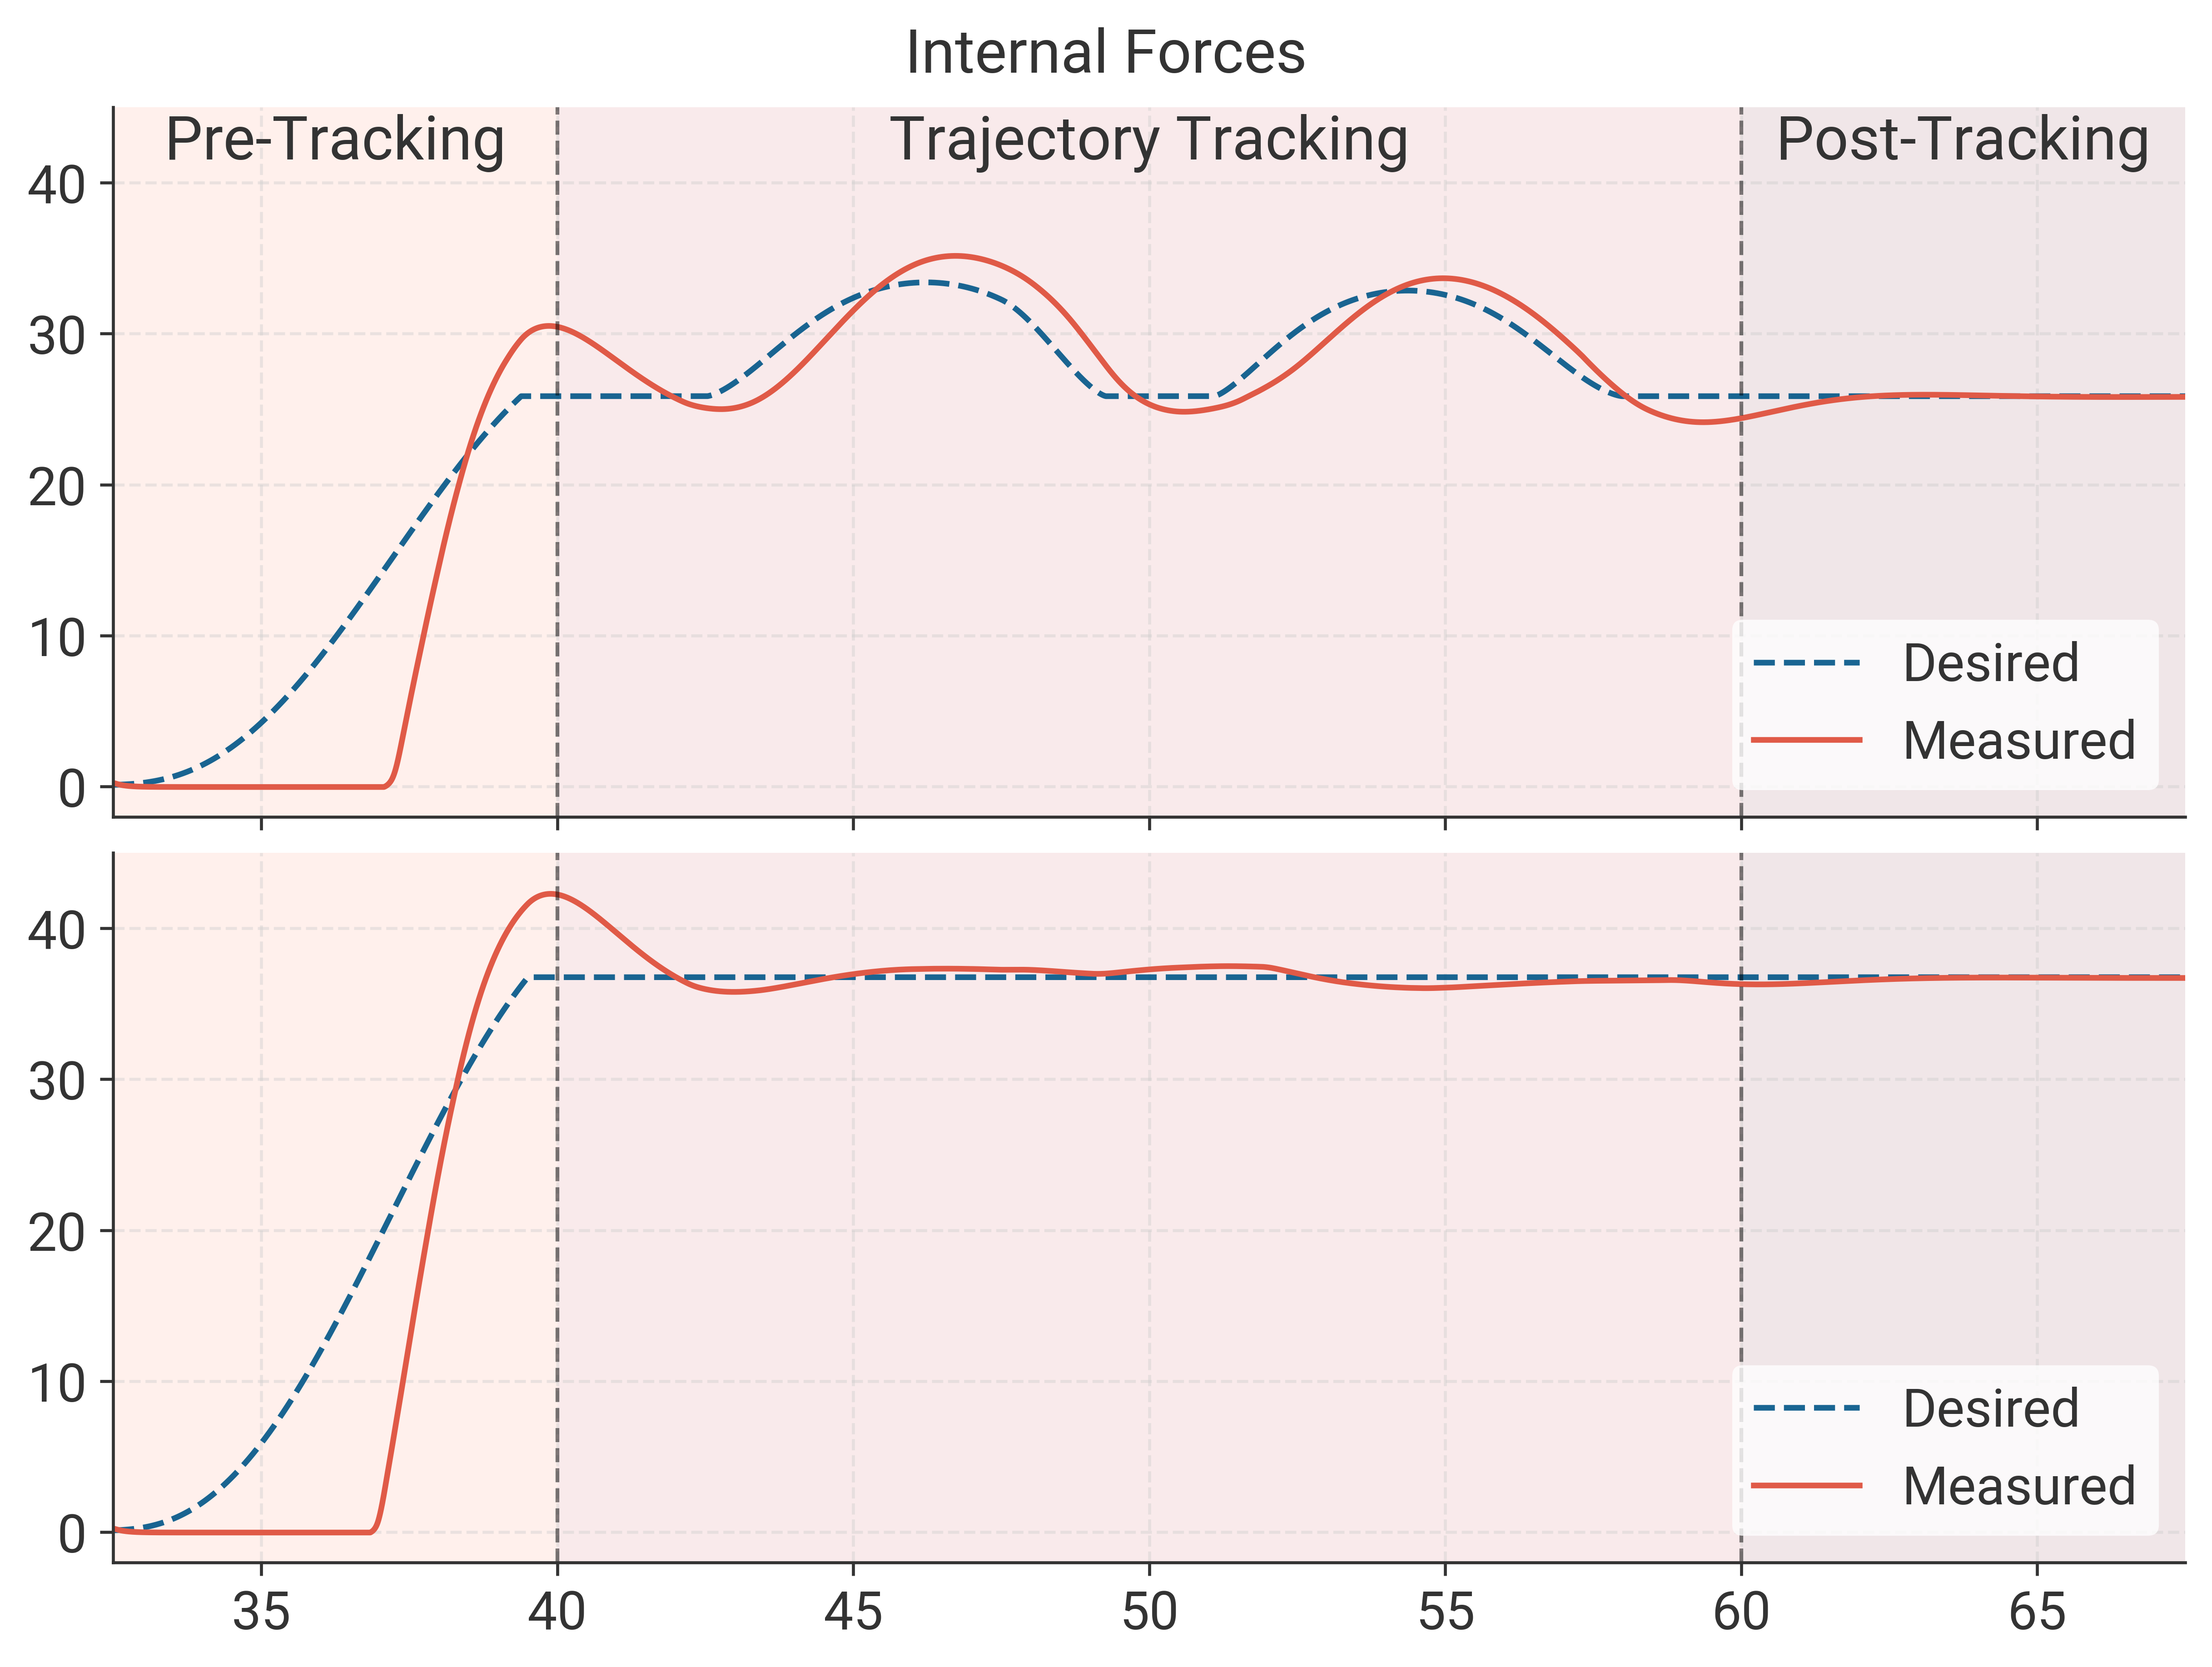
\includegraphics[width=0.85\columnwidth]{imgs/InternalForce.png}}
\caption{
 Comparison of the desired and measured internal grasping forces for two grasping strategies. 
(a) Proposed force-on-demand controller, which adaptively regulates the internal grasping force of the dual-arm system, increasing it only when required to ensure grasp stability 
(b) Baseline constant-force controller, where a fixed internal grasping force is maintained throughout the grasping task. 
The desired and measured internal forces are shown for both controllers.   
}
\label{InternalForceOnDemand}
\end{figure}

\begin{table}[htbp]
\caption{Power statistics and energy consumption for the single-cycle experiment}
\label{tab:power_statistics}
\centering
\small
\setlength{\tabcolsep}{3pt}
\begin{tabular}{|c|c|c|c|c|c|}
\hline
\textbf{Experiment} & \multicolumn{4}{c|}{\textbf{Power Statistics [W]}} & \textbf{Energy [J]} \\
\cline{2-5}
 & \textit{RMS} & \textit{Std} & \textit{Max} & \textit{Min} &  \\
\hline
Force On Demand & 12.57 & 2.81 & 15.36 & 6.11 & 428.78 \\
\hline
Constant Contact Forces & \makecell{\scriptsize(+14.9\%)} & \makecell{\scriptsize+16.6\%} & \makecell{\scriptsize+16.5\%} & \makecell{\scriptsize+8.9\%} & \makecell{\scriptsize+14.8\%} \\
\hline
\multicolumn{6}{l}{\scriptsize Values in parentheses: \% reduction relative to Force On Demand.}
\end{tabular}
\end{table}





\begin{figure}[htbp]
\centerline{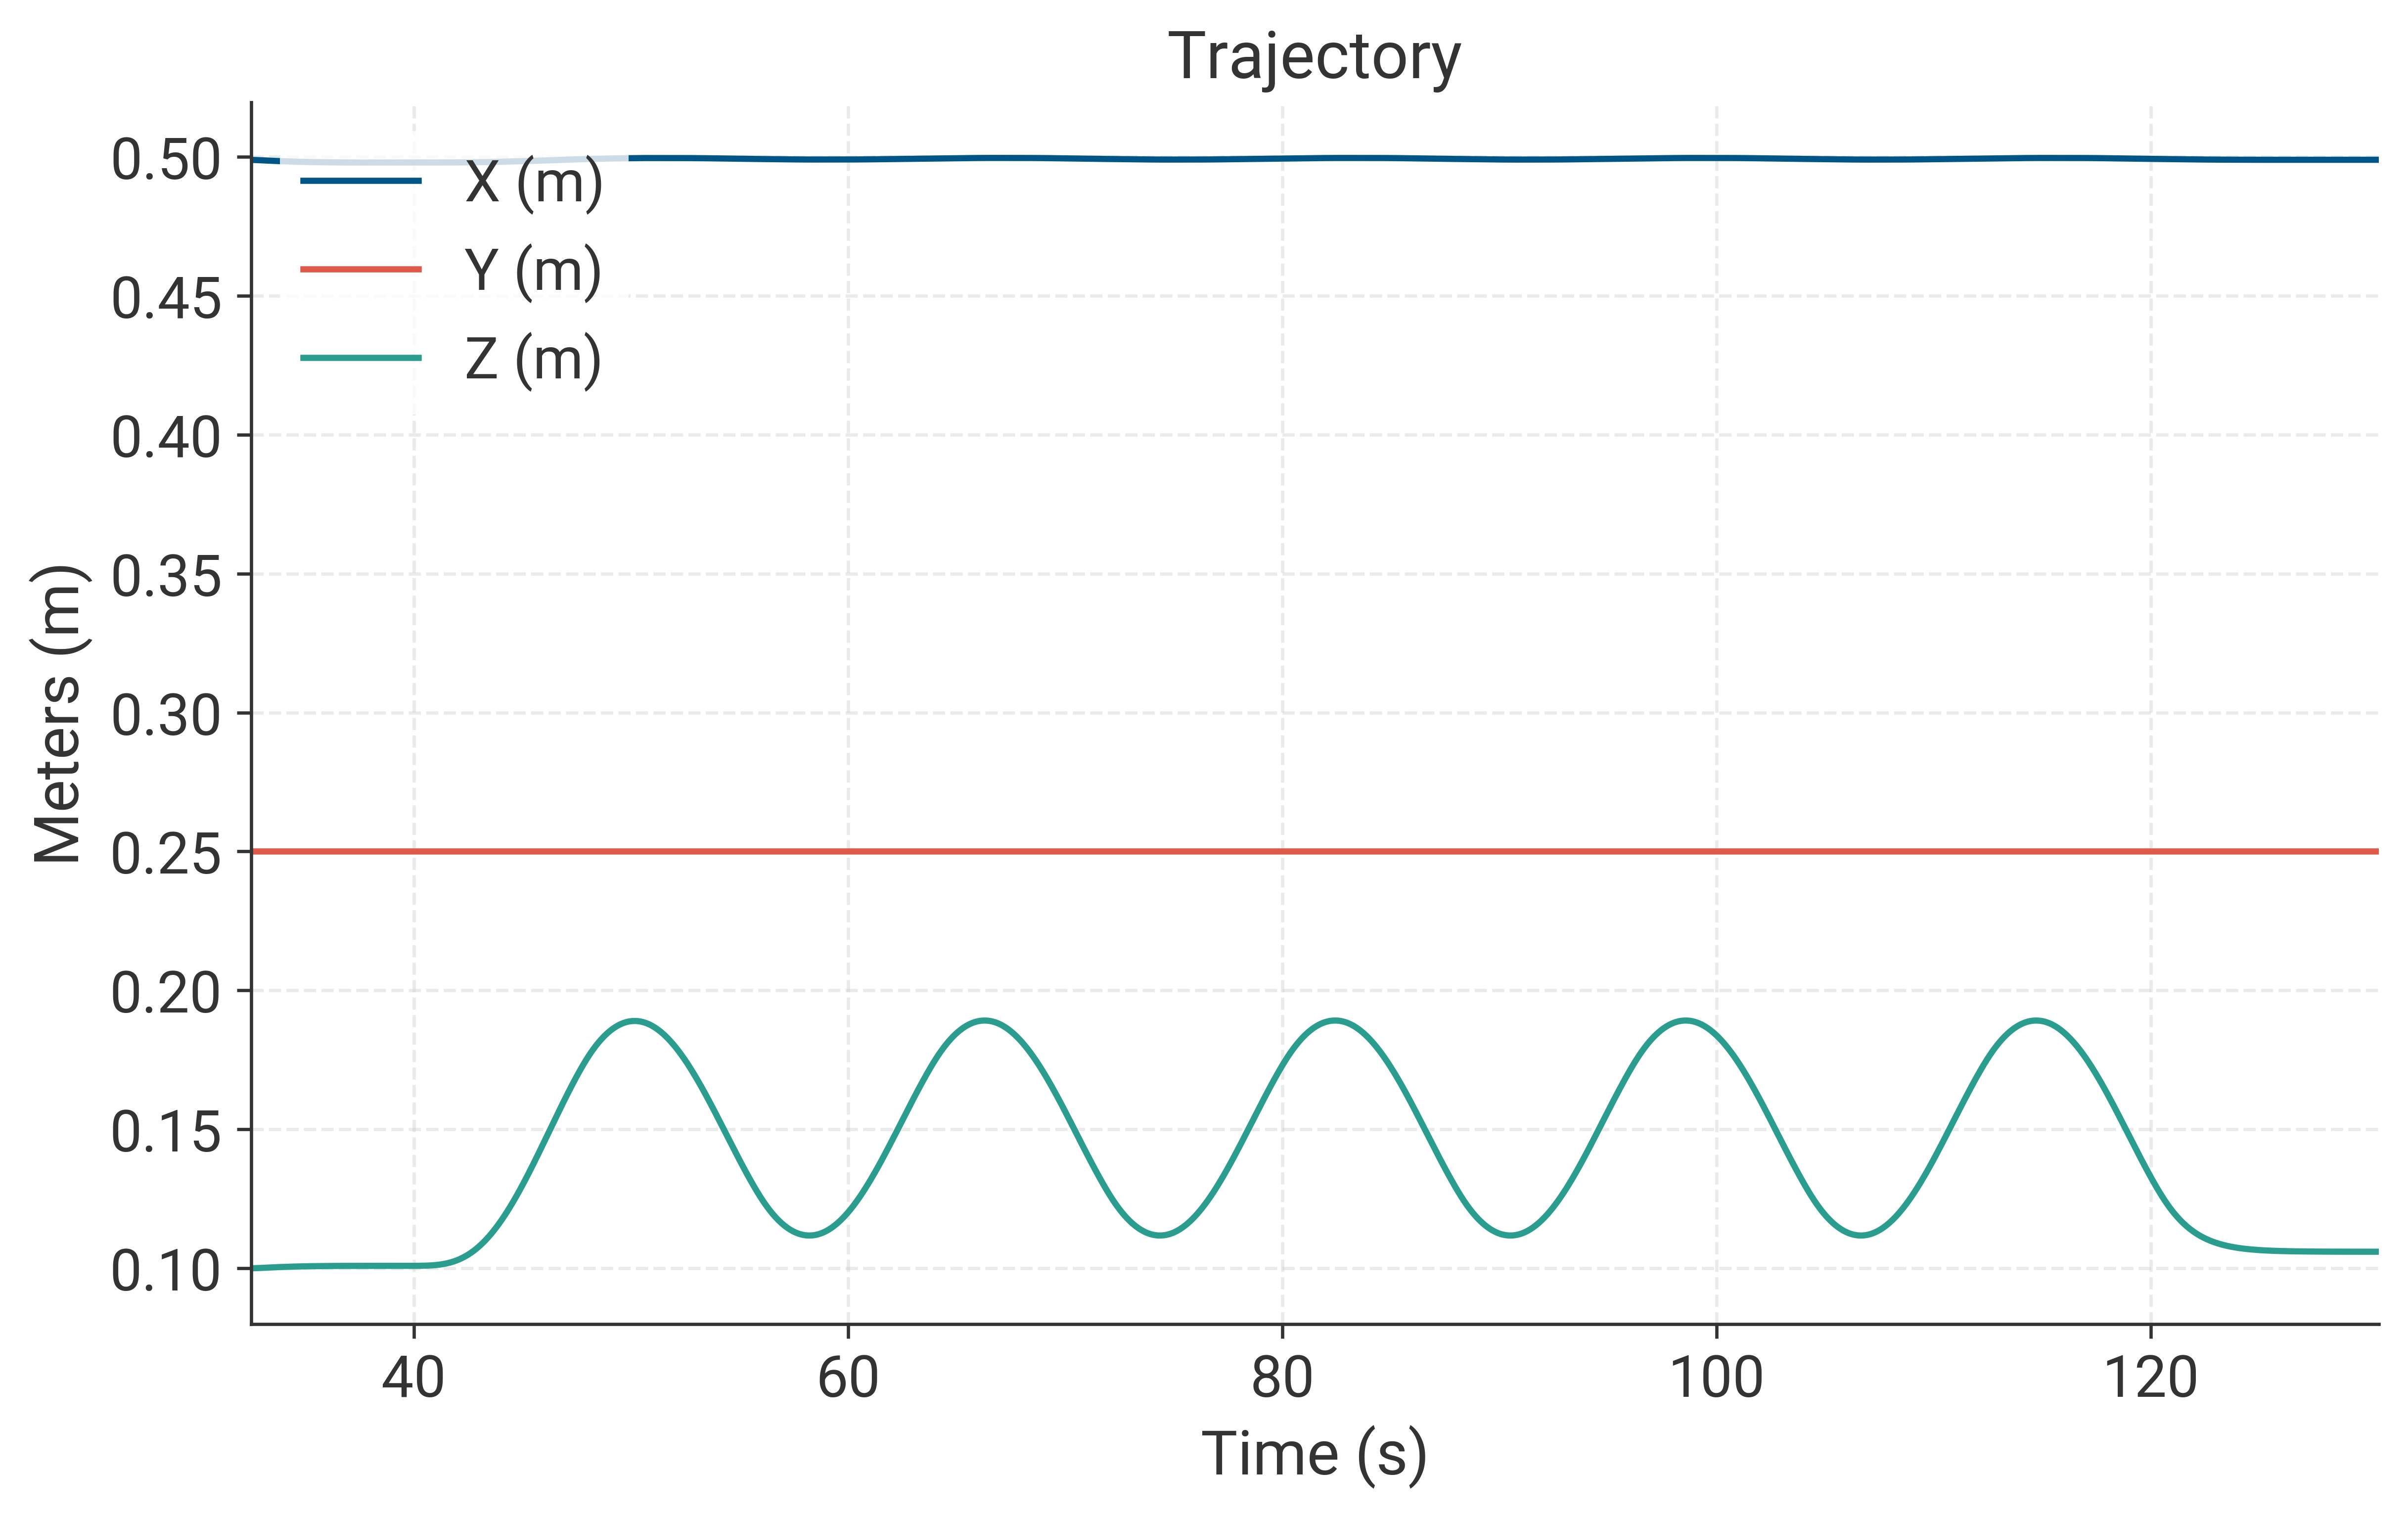
\includegraphics[width=0.85\columnwidth]{imgs/ObjectTrajecory_.png}}
\caption{Object trajectory during the cyclic waypoint-following experiment. The dual-arm system repeatedly traverses between 2 Waypoints for five consecutive cycles, demonstrating repeatable trajectory tracking.}
\label{ObjectTrajecoryFive}
\end{figure}

\begin{figure}[htbp]
\centerline{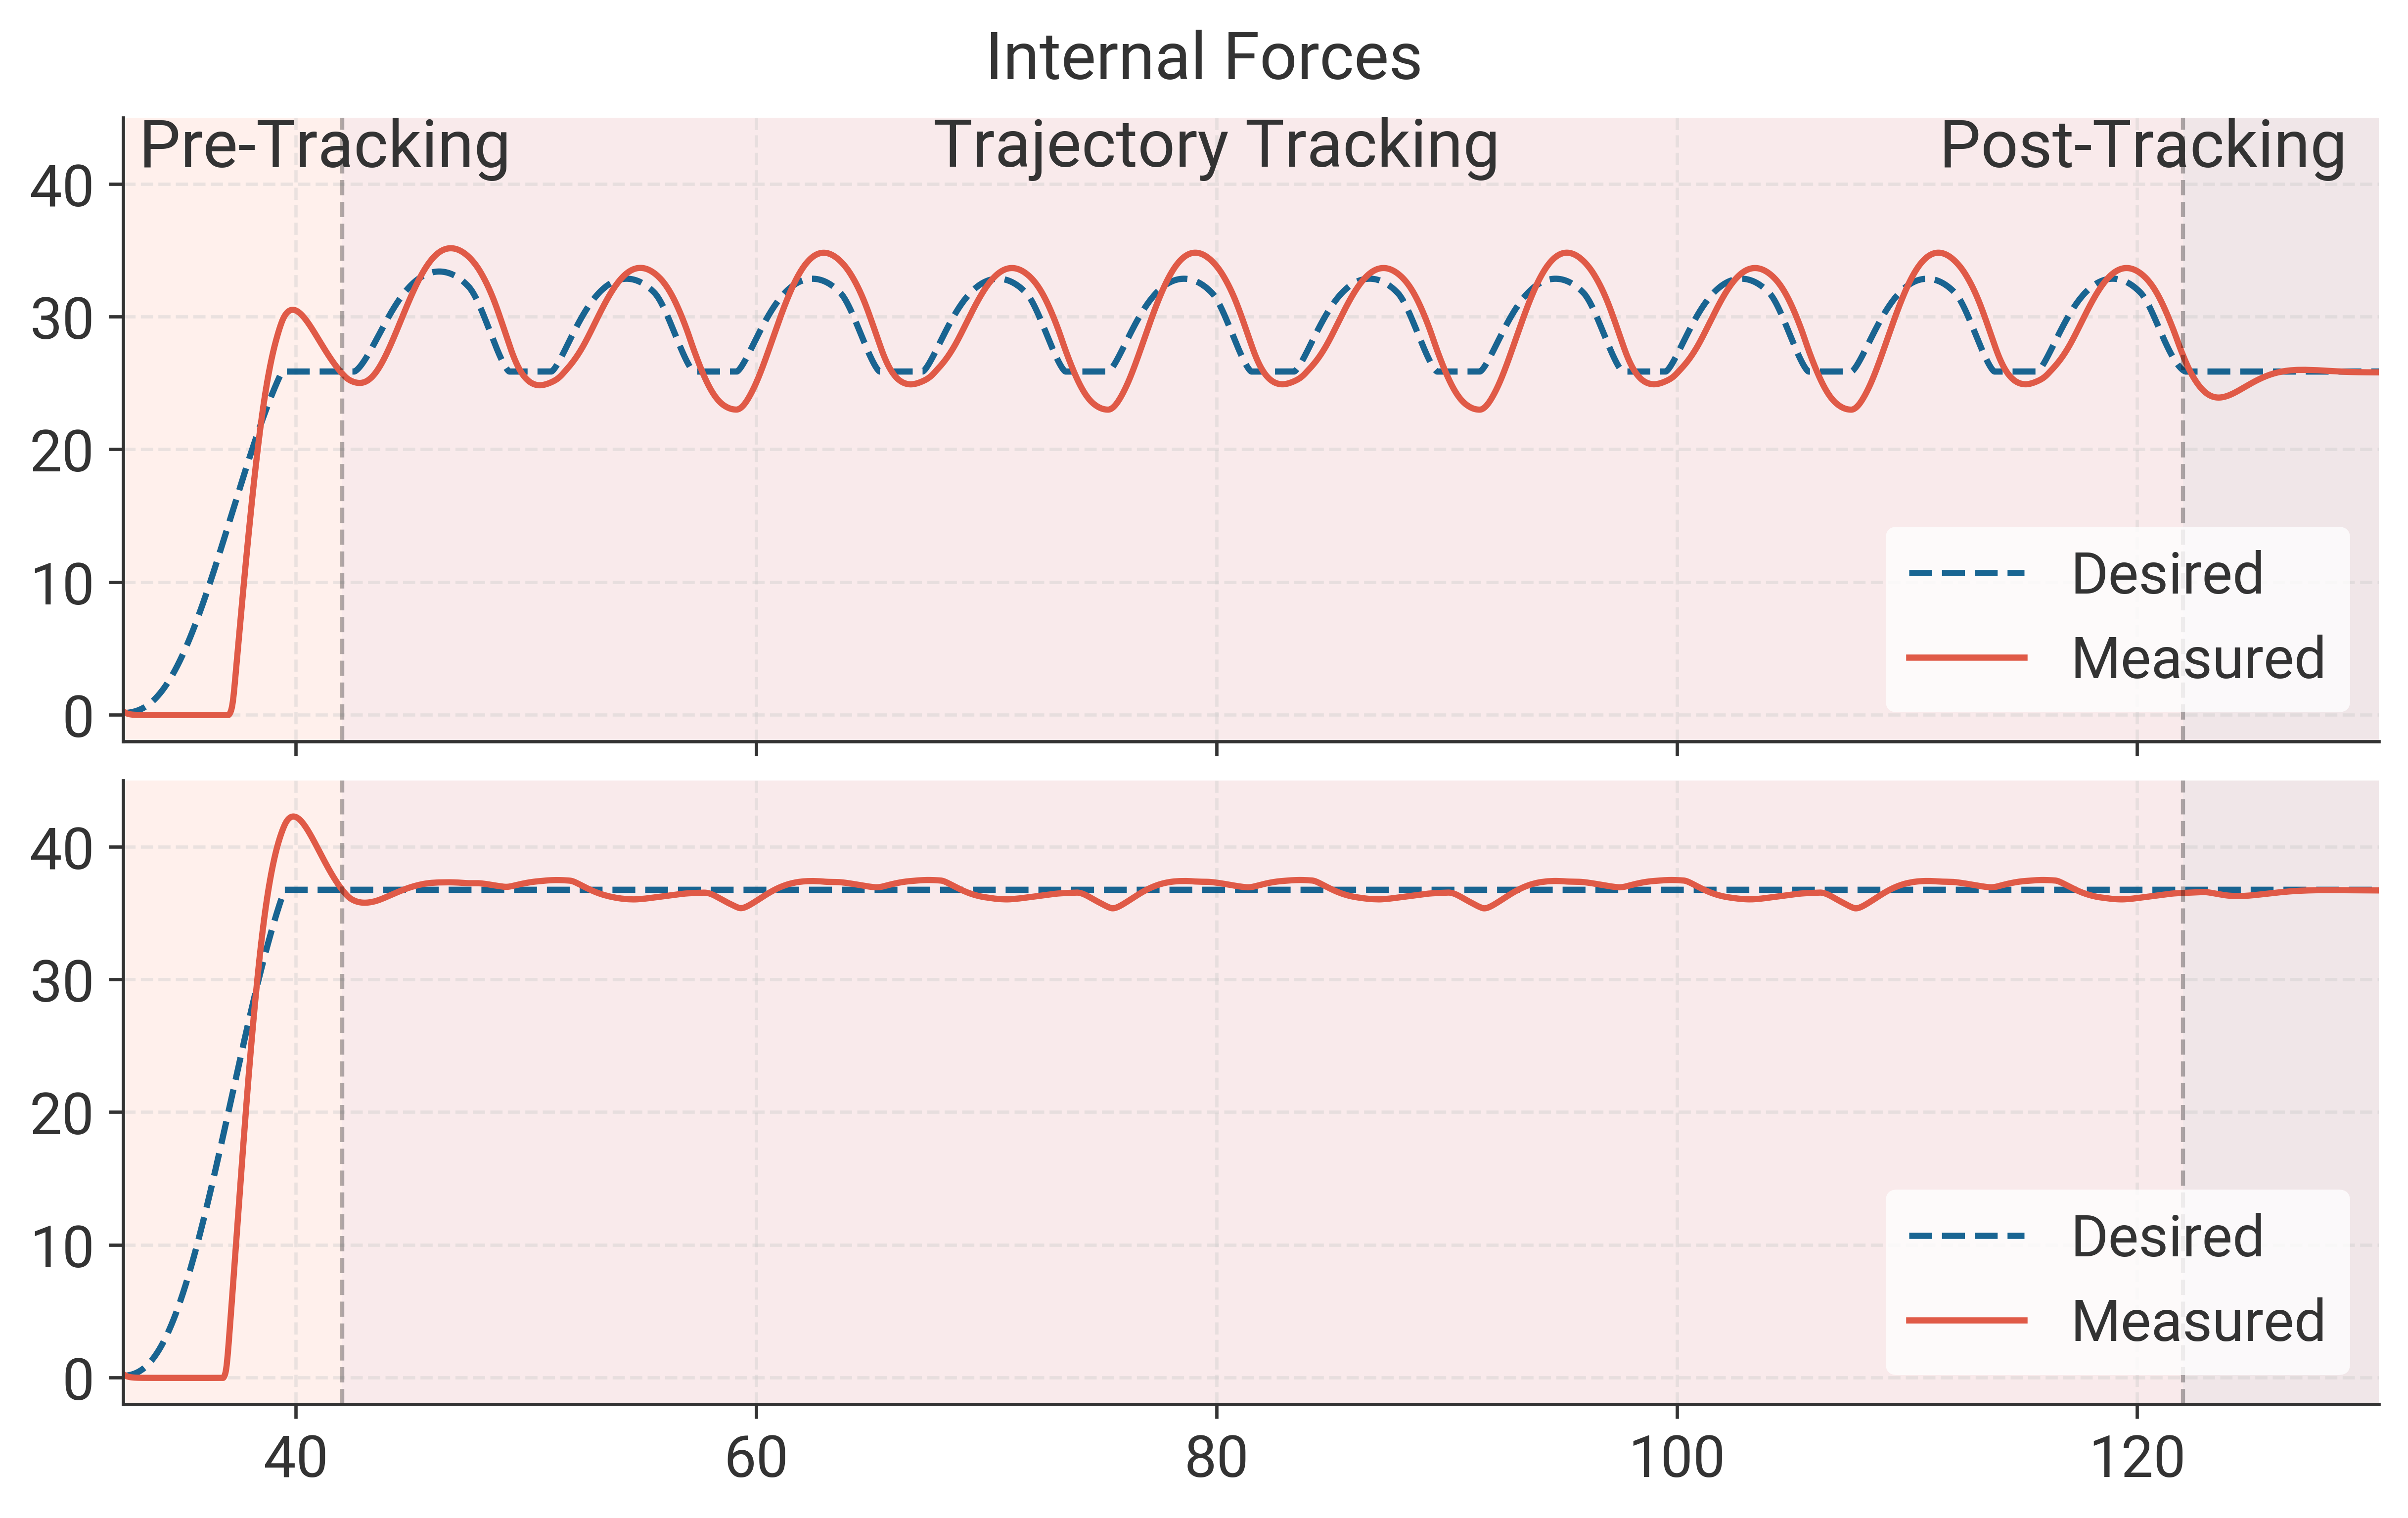
\includegraphics[width=0.85\columnwidth]{imgs/InternalForce_.png}}
\caption{Internal force tracking during the cyclic waypoint-following experiment. The dual-arm system repeatedly moves between Waypoints 1 and 2 for five consecutive cycles. (a) Proposed force-on-demand controller, which adaptively increases the internal grasping force only when necessary to enhance grasp stability. (b) Constant-force controller, which maintains a fixed internal grasping force throughout the task. The desired and measured internal forces are shown for comparison.}
\label{InternalForceOnDemandFive}
\end{figure}

\begin{table}[htbp]
\caption{Power statistics and energy consumption for the cyclic waypoint-following experiment}
\label{tab:power_statistics}
\centering
\small
\setlength{\tabcolsep}{3pt}
\begin{tabular}{|c|c|c|c|c|c|}
\hline
\textbf{Experiment} & \multicolumn{4}{c|}{\textbf{Power Statistics [W]}} & \textbf{Energy [J]} \\
\cline{2-5}
 & \textit{RMS} & \textit{Std} & \textit{Peak} & \textit{Min} &  \\
\hline
Force On Demand & 12.21 & 2.63 & 15.36 & 6.11 & 1168.53 \\
\hline
Constant Contact Forces & \makecell{14.09 \\ \scriptsize(+15.4\%)} & \makecell{2.65 \\ \scriptsize(+0.5\%)} & \makecell{17.90 \\ \scriptsize(+16.5\%)} & \makecell{6.66 \\ \scriptsize(+8.9\%)} & \makecell{1355.90 \\ \scriptsize(+16.0\%)} \\
\hline
\multicolumn{6}{l}{\scriptsize Values in parentheses: \% reduction relative to Force On Demand.}
\end{tabular}
\end{table}










\section{Discussion and Limitations}
\begin{itemize}
    \item Nonuniqueness of the internal/external decomposition: the weighted objective is a design choice, not ``the'' optimal split. State what it privileges (low effort vs.\ balance vs.\ torque margin) and how that choice was made.
    \item Linearized, one-cycle-lagged friction bound versus the exact friction cone: identify the operating regime in which this approximation may fail (e.g., fast tangential-force transients).
    \item Fixed versus state-driven weighting coefficients, \(\gamma_L\) and \(\gamma_R\): fixed weights are straightforward to justify but do not capture the instantaneous actuation capacity of each manipulator. \textbf{in future works} to present state-dependent weighting as the natural next step.
\end{itemize}
\section{Conclusion and Future Work}
\begin{itemize}
    \item \textbf{Summary:} The proposed framework combines QP-based dual-arm squeeze-force allocation, a motion-adaptive force-demand formulation, and a joint-torque-capacity-aware extension, and is validated experimentally on a dual \texttt{xArm7} platform.

    \item \textbf{Future Work:}
    \begin{itemize}
        \item \textbf{Hybrid feedforward--feedback force scheduling.} The proposed motion-adaptive scheduler is entirely measurement-driven, making it independent of the underlying trajectory generator and inherently robust to planner changes. However, because the demanded force is computed solely from the measured object velocity, it reacts only after the motion has occurred. An interesting extension is to combine the proposed scheduler with a trajectory-aware feedforward component. In such a formulation, the planned motion profile would provide a smooth anticipatory estimate of the required grasp force, while the measured object velocity would supply a corrective feedback term to compensate for disturbances, tracking errors, or deviations from the nominal trajectory. 
        \item Replace the fixed weighting coefficients \(\gamma_L\) and \(\gamma_R\) with state-driven weights based on online measures such as manipulability, joint-torque headroom, or actuator thermal state.
        \item Incorporate exact friction-cone handling through a second-order cone programming (SOCP) formulation, subject to real-time computational constraints.
    \end{itemize}
\end{itemize}


\section{References}
\begin{itemize}
    \item \textbf{Internal force decomposition / dual-arm QP allocation}
    \begin{itemize}
        \item Nahon, M., and Angeles, J. (1992) --- QP-based minimization of internal forces in cooperating manipulators.
        \item Kwon, W., and Lee, B.H. --- NLP/QP force-distribution scheme with normal-force constraints.
        \item Recent analysis on the nonuniqueness of nonsqueezing load distributions in cooperative manipulation (2023).
        \item Admittance-QP dual-arm cobot framework regulating internal/external efforts (BAZAR, 2017--2018).
        \item Recent HQP variants for mobile/free-floating dual-arm manipulation (2025--2026).
    \end{itemize}

    \item \textbf{Grasp/contact force optimization under friction}
    \begin{itemize}
        \item Buss, M., Hashimoto, H., and Moore, J.B. (1996), \emph{Dextrous Hand Grasping Force Optimization}, IEEE Transactions on Robotics and Automation.
        \item Kerr, J., and Roth, B.; Cheng, F., and Orin, D. --- polyhedral/linear friction-cone approximations.
        \item Recent work comparing SOCP and QP formulations for real-time grasp-force control (2026).
    \end{itemize}

    \item \textbf{Motion-adaptive / slip-driven grip force}
    \begin{itemize}
        \item Westling, G., and Johansson, R.S. (1984), \emph{Factors Influencing the Force Control During Precision Grip}, Experimental Brain Research, 53:277--284.
        \item Nature Machine Intelligence (2025) --- trajectory modulation versus grip-force modulation for slip control.
        \item Human hand-acceleration modulation study for slip prevention (2024).
        \item Reactive slip control via internal-force optimization for multifingered hands (2026 arXiv).
    \end{itemize}

    \item \textbf{Joint-space capacity-aware allocation}
    \begin{itemize}
        \item Classical minimum-norm / weighted-pseudoinverse torque allocation for redundant and multi-arm systems.
        \item Whole-body and multi-contact QP controllers with torque- or actuation-margin-aware cost terms (locomotion / multi-contact force-distribution literature).
    \end{itemize}

    \item \textbf{Contact-state transition / hybrid position-force control}
    \begin{itemize}
        \item Raibert, M.H., and Craig, J.J. (1981) --- classical orthogonal position/force subspace hybrid control.
        \item Recent orthogonal interaction-frame decomposition for contact-rich manipulation (2026).
        \item Smooth controller blending / gain interpolation across contact-state transitions (changing-contact manipulation frameworks).
    \end{itemize}

    \item \textbf{Impact-aware contact establishment (background only)}
    \begin{itemize}
        \item van Steen, J.J., Coşgun, A., van de Wouw, N., and Saccon, A., \emph{Dual-Arm Impact-Aware Grasping through Time-Invariant Reference Spreading Control}, IFAC-PapersOnLine, 2023.
        \item van Steen, J.J., van den Brandt, G., van de Wouw, N., Kober, J., and Saccon, A., \emph{QP-Based Reference Spreading Control for Dual-Arm Robotic Manipulation with Planned Simultaneous Impacts}, IEEE Transactions on Robotics, 2024.
        \item Arita, H., Nakamura, H., Fujiki, T., and Tahara, K. --- \emph{Smoothly Connected Preemptive Impact Reduction and Contact Impedance Control}, 2022/2023.
        \item Khatib, O. --- effective/reflected mass in operational-space control.
        \item Wang, Y., Dehio, N., Tanguy, A., and Kheddar, A., \emph{Impact-Aware Task-Space Quadratic-Programming Control}, International Journal of Robotics Research, 2023.
    \end{itemize}
\end{itemize}

\bibliographystyle{IEEEtran}
\bibliography{references}








\end{document}

